\documentclass[addpoints]{exam}

\usepackage{amsmath}
\usepackage{hyperref}
\usepackage{tikz}
\usepackage{graphicx}
\usepackage{pseudocode}

% Header and footer.
\pagestyle{headandfoot}
\runningheadrule
\runningfootrule
\runningheader{CS 201 DS II}{Homework 3}{Spring 2018}
\runningfooter{}{Page \thepage\ of \numpages}{}
\firstpageheader{}{}{}

\qformat{{\large\bf Exercise \thequestiontitle}\hfill[\totalpoints\ points]}
\boxedpoints
\printanswers

\title{\textbf{\tt Habib University}\\ \textbf{\tt CS 201 Data Structures II}\\ \textbf{\tt Spring 2018}}
\author{\textbf{\tt Emad Bin Abid - Saman Gaziani}\\ {\tt $Team: hw-3-ea02893-sg02494-3$}}
\date{\textbf{\tt Homework 3}\\ \textbf{\tt Submitted: February 23\textsuperscript{rd}, 2018}}

\begin{document}
\maketitle

\begin{questions}

  \titledquestion{12.4}[5]
  Let $G$ be an undirected graph. We say $G$ is {\it connected} if, for every pair of vertices $i$ and $j$ in $G$, there is a path from $i$ to $j$ (since $G$ is undirected, there is also a path from $j$ to $i$). Show how to test if $G$ is connected in $O(n + m)$ time.
  \begin{solution}
  	This question can be answered by using any of the two famous graph traversal algorithms; Breadth First Search (BFS) and Depth First Search (DFS). Both algorithms have the same time complexity so we can use any of them to answer the given question. Let's consider $BFS$ for the given scenario. \\ \\
  	We know that a $BFS$ maintains a queue/set ($q$) of visited nodes in it. While carrying out this search, we know by algorithm, that it takes $O(m)$ time to execute, where $m$ is the number of edges in  graph $G$. To show if $G$ is connected or not, we check the queue $q$ which contains all the visited nodes during the traversal. If we find each node of original set of vertices $V$ in $q$ we say that $G$ is connected. We can also compare the lengths of $V$ and $q$. If $\left|V\right| = \left|q\right|$, we say that $G$ is connected. The small operation happens in $O(n)$ time. \\ \\
  	Hence, the total cost for entire operation is $O(n+m)$.
  	%Before answering to the given question, we make some assumptions and on the basis of these assumptions we put forward the required solution. Let $V$ be the set of vertices and $E$ be the set of edges for a given graph $G$. Furthermore, let $n=\left|V\right|$ and $m=\left|E\right|$.\\ \\
  	%Before constructing edges in $G$, we map the node identities to natural numbers. We traverse through the set of vertices $V$ and create a new set $V_0$ which has a continuous sequence of natural numbers as the node identity. The cost of this process is $O(n)$.\\ \\
  	%Next, we find the maximum ($max$) from the set $V_0$. This process also runs in $O(n)$ time. Up till now the cost of operations has appeared to be $O(2n)$, which is actually $O(n)$ in asymptotic analysis. We now traverse through the set of edges $E$ linearly and for each entry we check if the tuple has both the nodes greater than or equal to $1$ and less than or equal to $max$.\\ Mathematically, \\
  	%\begin{center}
  		%$\forall i \forall j ((i \geq 1 \wedge i \leq max) \wedge (j \geq 1 \wedge j \leq max) \rightarrow true)$ where $i, j \in V_0$.
  	%\end{center}
  	%The above process takes $O(m)$ time to execute. If the above process returns true, we just compare length of set $E$ to the square of length of set $V_0$. Since there is not any restriction that $i \neq j$ so if $m=n^2$ then we know that the graph is connected. The process took $O(m+n)$ time to execute. Hence, the desired result is achieved. 
    \end{solution}
\pagebreak

  \titledquestion{12.5}[5]
  Let $G$ be an undirected graph. A {\it connected-component labelling} of $G$ partitions the vertices of $G$ into maximal sets, each of which forms a connected subgraph. Show how to compute a connected component labelling of $G$ in $O(n + m)$ time.
  \begin{solution}
  	We will follow the same approach in this question which we followed in the previous exercise. We will again use a breadth first traversal technique to find the {\it connected component labelling} of the graph $G$. \\ \\
  	We know that $BFS$ maintains a queue/set ($q_0$) of visited nodes. Let's say that $V$ is a set of vertices in $G$. We pick any random node from $V$ and apply $BFS$ on $G$ in reference to the selected node. After completion of $BFS$, we have some nodes present in $q$. We check whether all the nodes of $V$ are in $q_0$ or not. If they are present in $q_0$, then we simply know that the given graph is a single component and has only one entry in connected component labelling. If the check returns false then we pick any random node amongst the remaining (unvisited) nodes of $V$. We again apply a $BFS$ in reference to the newly selected node and store its visited nodes in a new queue/set $q_1$. We again place a check on whether the nodes are still visited or not. \\
  	We repeat this process unless the check on set $V$ returns true. The truth value $T$ of returning statement indicates that $q_0 \cup q_1 \cup ... \cup q_n = V$ and each $q_i$ is represents a distinct connected component labelling; where $0 \leq i \leq n$.\\ \\
  	Since each $BFS$ takes $O(m+n)$ time to execute, hence the whole process will run in $O(m+n)$ time because the number of times the $BFS$ works is some constant $c$. 
  \end{solution}
\pagebreak

  \titledquestion{12.7}[10]
  We say that a directed graph $G$ is {\it strongly-connected} if, for every pair of vertices $i$ and $j$ in $G$,there is a path from $i$ to $j$. Show how to test if $G$ is strongly-connected in $O(n + m)$ time.
  \begin{solution}
  	In this question, we follow the same procedure as in Exercise $12.4$ with a slight modification in the procedure. The procedure adopted is discussed below. \\ \\
  	We again use Breadth First Search ($BFS$) for this question. We know that a $BFS$ maintains a queue, $q$, of visited nodes in it. While carrying out this search, we know by algorithm, that it takes $O(m)$ time to execute, where $m$ is the number of edges in  graph $G$. To show if $G$ is strongly-connected or not, we divide the process into two stages. \\ \\
  	i. In the first stage, we check the queue/set ($q$) which contains all the visited nodes during the normal traversal. If we find each node of original set of vertices $V$ in $q$ we say that $G$ is connected only in this direction. In other words, we have concluded that the vertex $S$ can reach every other node in $G$; where $S$ is the vertex on which we began the $BFS$ traversal. \\ \\
  	ii. Previously we found out that $S$ can reach every other node in the graph. In the second stage, we try to find whether $S$ is reachable from every other node or not. For this purpose we reverse the direction of every edge in $G$. This work can be done in $O(m)$ time since we traverse through the set of edges linearly and swapping the values of each tuple. After this we again apply $BFS$ from the same node $S$. If we find every node which is in $V$ also in the queue $visited$, we say that $S$ is reachable from every other node in $G$. \\ \\
  	Therefore, by modifying the procedure a bit we have found whether a directed graph is strongly-connected or not. 
  	
  	The costs involved in this process are:\\
  	\begin{center}
  		$O(m+n+m+m+n)$\\
  		$O(3m+2n)$\\
  	\end{center}
  	Asymptotically, \\
  	\begin{center}
  		$O(m+n)$
  	\end{center}
  	Hence, the total cost for entire operation is $O(n+m)$.
  \end{solution}
\pagebreak

  \titledquestion{12.10*}[15]
  A {\it universal sink} in a graph $G$ is a vertex that is the target of $n-1$ edges and the source of no edges.\footnote{A universal sink, $v$, is also sometimes called a {\it celebrity}: Everyone in the room recognizes $v$, but $v$ doesn't recognize anyone else in the room.} Design an algorithm that tests if a graph $G$, represented as an AdjacencyMatrix, has a universal sink. Your algorithm should run in $O(n)$ time.\\
  \underline{Hint}: Draw a few graphs with a universal sink and observe their adjacency matrix.
  \begin{solution}
  	The idea is to find a {\it universal sink}, $S$, for a given graph $G$ in $O(n)$ time where $n$ is the number of nodes in $G$. We start with the eliminating approach. We first eliminate those nodes which do not qualify for the sink. This process will be efficiently done in $O(n)$ time by traversing over the matrix smartly. Next we check the row entries of the node which so far qualifies for the {\it universal sink} in $O(n)$ time. Finally, we check the column entries of that same node to check if it is actually a {\it universal sink}. This process will also be done in $O(n)$ time. Asymptotically, the whole process will be carried out in $O(n)$ time. 
  	
  	\begin{pseudocode}{UniversalSink}{G, n}
  		\label{Universal Sink}
  		\COMMENT{Finds a universal sink in a graph $G$ in $O(n)$ time if it exists.}\\
  		
  		${\tt The idea of this algorithm is taken from \underline{geeksforgeeks}. The pseudocode is}$\\ ${\tt however self-generated.}$\\ \\
  		
  		\PROCEDURE{find\_universal\_sink}{$G$}
  		i \GETS 0 \\
  		j \GETS 0 \\
  		\WHILE i < n \AND j < n\DO 
  		\BEGIN
  		\IF i \neq j
  		\THEN 
  			\BEGIN
  			\IF G[i][j] == 0 
	  		\THEN i = i + 1
	  		\ELSE j = j + 1\\
	  		\END \\
	  	\ELSE i = i + 1
	  	\END \\ \\
	  	
	  	\IF j > i
	  	\THEN j = i
	  	\ELSE i = j\\ \\
	  	
	  	destination \GETS i \\ \\
	  	
	  	\FOR counter \GETS i \TO n-1 \DO
	  	\BEGIN
	  		\IF G[i][j] == 0 
	  		\THEN i = i + 1
	  		\ELSE 
	  		\RETURN{false}
	  	\END \\ \\
	  	
	  	\FOR counter \GETS j \TO n-1 \DO
	  	\BEGIN
	  	\IF G[i][j] == 1 \AND i \neq j
	  	\THEN j = j + 1
	  	\ELSE 
	  	\RETURN{false}
	  	\END \\ \\
	  	
	  	\RETURN{destination}
  		\ENDPROCEDURE
  	\end{pseudocode}
  \end{solution}
\pagebreak

  \qformat{{\large\bf \thequestiontitle}\hfill[\totalpoints\ points]}

  \titledquestion{Graph Complement}[15]

  The complement of an undirected graph $G$ is a graph $H$ on the same vertices such that two distinct vertices of $H$ are adjacent (connected by an edge) if and only if they are not adjacent in $G$.\footnote{\url{https://en.wikipedia.org/wiki/Complement_graph}} Prove that if $G$ is not a connected graph then its complement $H$ is a connected graph.
  \begin{solution}
  	In an undirected graph, there is only one possibility when the graph is not connected. And that is when it has components in it.\\ \\ 
  	\textbf{{I - Proof by Intuition:}} \\ \\
	Suppose that $G$ is not connected graph and is composed of $n$ components such that $n_1, n_2, n_3, ..., n_n$ are the $n$ sub-graphs of $G$. \\ \\
	The graph $G$ for now is not connected and contains components but in its inverse graph $H$, the components will get connected to each other because where ever there was not an edge between two nodes, an edge is created there in the inverse graph. Although the existing edges in $G$ with in a component will get removed, but still, they will be connected undirectly through the newly created edges of the nodes of other components. \\ \\
	The above stated proof is demonstrated with an example shown below: \\ \\ Consider a graph $G$ with nodes $0, 1, 2, 3, 4, 5, 6, 7, 8, 9, 10$. The graph $G$ is connected in such a way that it has three sub-graphs (components). The nodes $0, 1, 2$ form first component, the nodes $3, 4, 5, 6$ form second component and the nodes $7, 8, 9, 10$ form third component. The graph $G$ is visually represented below: 
	\begin{center}
		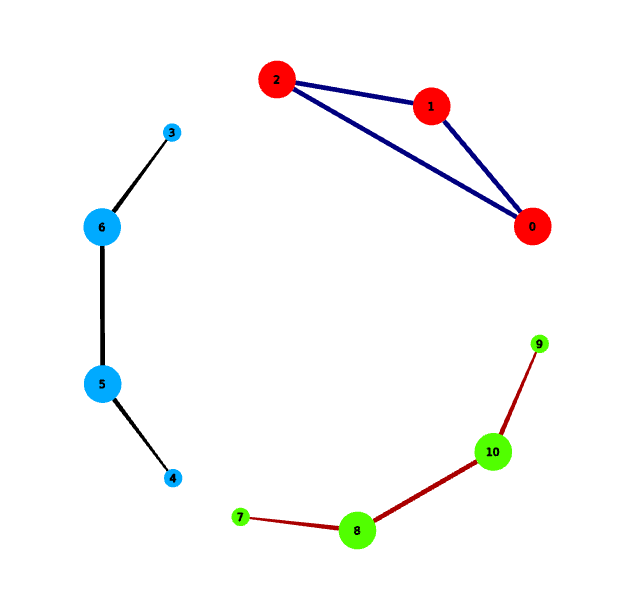
\includegraphics[scale=0.5]{original_graph_2}\\
	\end{center}
\pagebreak
	We now produce the complement $H$ of graph $G$. The visuals of graph's complement are shown below. The visuals clearly show that the graph is now connected; since there exists a path from each node to every other node. 
	\begin{center}
		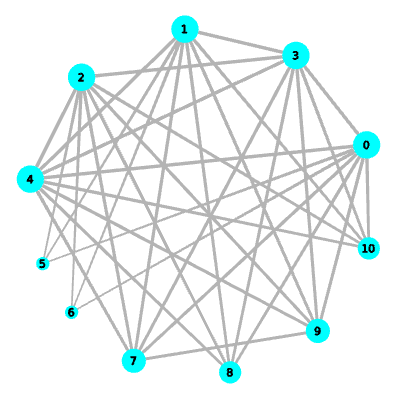
\includegraphics[scale=0.8]{complement_graph_2}\\
	\end{center}
	Hence, it is proved that if a graph $G$ is un-connected i.e. it has more than one component then $G$'s complement $H$ will always be connected i.e. a single component. \\ \\
	\textbf{II - Proof by Induction:}\\ \\
	In order to prove that if $G$ is not connected then its complement $H$ must be connected by induction, we assume a base case where $\left|V\right|=2$. \\ \\
	\textbf{Base Case:}
	\begin{center}
		$\left|V\right|=2$
	\end{center} 
	In base case $G$ has two vertices, $V_1$ and $V_2$. $V_1$ is not connected to $V_2$ means that the graph has two components. If we take complement of this graph, $V_1$ gets connected to $V_2$. Hence, the base case holds. \\ \\
	\textbf{Inductive Hypothesis:}\\
	Assuming that the statement is true for $\left|V\right|=k$. Let's say that $k-1$ vertices are connected to each other and only $k$ is an isolate. The graph has more than one component. If we take complement of $G$, all the $k-1$ nodes get connected to the $k_{th}$ isolate node and hence get connected as a single component via that $k_{th}$ node. Hence the hypothesis is valid to be assumed. \\ \\
	\textbf{Inductive Step:}\\
	Considering the same scenario as in Inductive Hypothesis, we have to prove that if the proof is valid for $k_{th}$ node then it must also be valid for $(k+1)_{th}$ node. Now we have three components in $G$ namely \{$0, 1, 2, ..., k-1$\}, $k$ and $k+1$. The component \{$0, 1, 2, ..., k-1$\} now has two $k_{th}$ nodes; the node $k$ and the node $k+1$. It follows from the inductive hypothesis that the proof holds valid for $k$ nodes. Since in this step there are two $k$ nodes for \{$0, 1, 2, ..., k-1$\} component, therefore, the proof holds valid for \{$0, 1, 2, ..., k-1$\} and $k$, plus, for \{$0, 1, 2, ..., k-1$\} and $k+1$. Eventually leading to the validity of \{$0, 1, 2, ..., k-1$\}, $k$ and $k+1$. 
  \end{solution}
\pagebreak

  \titledquestion{Topological Sort}

  A {\it topological sort} or {\it topological ordering} of a directed graph is a linear ordering of its vertices such that for every directed edge $(u,v)$ from vertex $u$ to vertex $v$, $u$ comes before $v$ in the ordering.\footnote{\url{https://en.wikipedia.org/wiki/Topological_sorting}}

  Find a topological ordering of each of the following two graphs.

  \begin{parts}
    \part[5]
    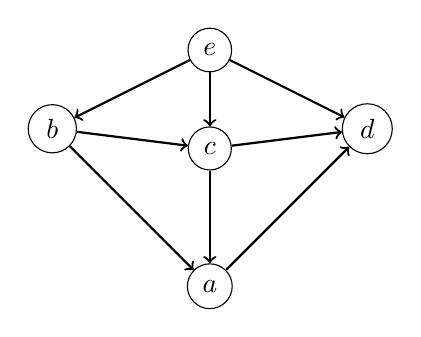
\begin{tikzpicture}
      \foreach \pos/\name in { {(2,0)/a}, {(0,2)/b}, {(2,1.75)/c}, {(4,2)/d}, {(2,3)/e}}
      \node[circle,draw] (\name) at \pos {$\name$};
      \foreach \source/ \dest in {a/d, c/d, c/a, b/a, b/c, e/b, e/c, e/d}
      \path[draw,thick,->] (\source) -- (\dest);
    \end{tikzpicture}
    \begin{solution}
    	In order to do a {\it topological sort} on graphs, we first check the two conditions:\\
    	i. the graph should be acyclic i.e. it should not contain any cycles.\\
    	ii. the graph should be directed.\\ \\
    	Since the given graph satisfies both conditions, we apply $DFS$ for topological sorting. \\ \\
    	Let there be two stacks; {\it process} and {\it completed} and a set; {\it visited}. Every time we visit a new node, we put that node to the set {\it visited}. We push in {\it process} every time we find the children of current node. Lastly, if the current node has no un-visited children we put that node in the stack {\it completed}.\\ \\ 
    	\textbf{Working:}
    	Starting off with any node which has $indegree = 0$. Let's say $e$. \\ \\
    	Pushing $e$ and its children in {\it process}: \\
    	\begin{center}
    		$process$ = [$e, b, c, d$]\\
    		$completed$ = [ ]\\
    		$visited$ = \{ \}\\
    	\end{center}
    	Pop $d$ and add it to {\it visited}: \\
    	\begin{center}
    		$process$ = [$e, b, c$]\\
    		$completed$ = [ ]\\
    		$visited$ = \{$d$\}\\
    	\end{center}
    	Since $d$ has no un-visited node, we push it in $completed$.\\
    	\begin{center}
    		$process$ = [$e, b, c$]\\
    		$completed$ = [$d$]\\
    		$visited$ = \{$d$\}\\
    	\end{center}
    	Once pushing to $completed$ is made, we go back to $process$. Push $c$'s children to {\it process}. \\
    	\begin{center}
    		$process$ = [$e, b, a, d$]\\
    		$completed$ = [$d$]\\
    		$visited$ = \{$d, c$\}\\
    	\end{center}
    	$d$ is already in $visited$. So,\\
    	\begin{center}
    		$process$ = [$e, b, c, a$]\\
    		$completed$ = [$d$]\\
    		$visited$ = \{$d, c$\}\\
    	\end{center}
    	$a$ does not have any un-visited child. So,\\
    	\begin{center}
    		$process$ = [$e, b, c$]\\
    		$completed$ = [$d, a$]\\
    		$visited$ = \{$d, c, a$\}\\
    	\end{center}
    	Again, go to $process$. We do not have any un-visited nodes of $c$. So, \\
    	\begin{center}
    		$process$ = [$e, b$]\\
    		$completed$ = [$d, a, c$]\\
    		$visited$ = \{$d, c, a$\}\\
    	\end{center}
    	We again go to $process$:\\
    	\begin{center}
    		$process$ = [$e, a, c$]\\
    		$completed$ = [$d, a, c, b$]\\
    		$visited$ = \{$d, c, a, b$\}\\
    	\end{center}
    	In the next step: \\
    	\begin{center}
    		$process$ = [$e$]\\
    		$completed$ = [$d, a, c, b$]\\
    		$visited$ = \{$d, c, a, b$\}\\
    	\end{center}
    	Finally,\\
    	\begin{center}
    		$process$ = [ ]\\
    		$completed$ = [$d, a, c, b, e$]\\
    		$visited$ = \{$d, c, a, b, e$\}\\
    	\end{center}
    	Hence, our topological sort sequence is generated by popping elements from the stack {\it \textbf{completed}}.\\
    	\begin{center}
    		{\it \textbf{e, b, c, a, d}}
    	\end{center} 
    \end{solution}
    \part[10]

    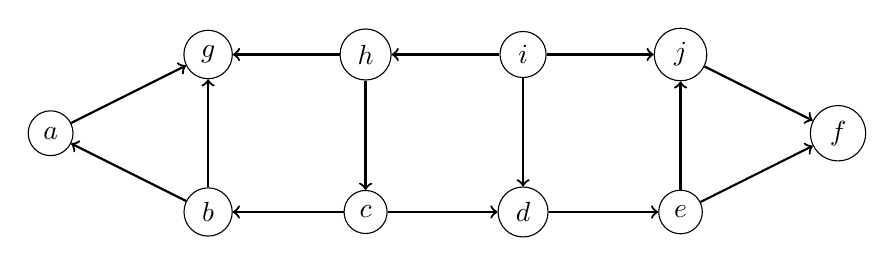
\begin{tikzpicture}
      \foreach \pos/\name in {{(0,1)/a}, {(2,0)/b}, {(4,0)/c}, {(6,0)/d}, {(8,0)/e}, {(10,1)/f}, {(2,2)/g}, {(4,2)/h}, {(6,2)/i}, {(8,2)/j}}
      \node[circle,draw] (\name) at \pos {$\name$};
      \foreach \source/ \dest in {b/a, a/g, b/g, c/b, c/d, d/e, e/f, e/j, h/g, i/h, h/c, i/d, i/j, j/f}
      \path[draw,thick,->] (\source) -- (\dest);
    \end{tikzpicture}
    \begin{solution}
    	In order to do a {\it topological sort} on graphs, we first check the two conditions:\\
    	i. the graph should be acyclic i.e. it should not contain any cycles.\\
    	ii. the graph should be directed.\\ \\
    	Since the given graph satisfies both conditions, we apply $DFS$ for topological sorting. \\ \\
    	Let there be two stacks; {\it process} and {\it completed} and a set; {\it visited}. Every time we visit a new node, we put that node to the set {\it visited}. We push in {\it process} every time we find the children of current node. Lastly, if the current node has no un-visited children we put that node in the stack {\it completed}.\\ \\
    	\textbf{Working: } The whole process has been explained in part (a). In this part, only steps will be demonstrated. \\ \\
    	Starting off with any node which has $indegree = 0$. Let's say $i$. \\ \\
    	(i)
    	\begin{center}
    		$process$ = [$i, h, d, j$]\\
    		$completed$ = [ ]\\
    		$visited$ = \{ \}\\
    	\end{center}
    	(ii)
    	\begin{center}
    		$process$ = [$i, h, d, j, f$]\\
    		$completed$ = [ ]\\
    		$visited$ = \{$j$\}\\
    	\end{center}
    	(iii)
    	\begin{center}
    		$process$ = [$i, h, d, j, f$]\\
    		$completed$ = [ ]\\
    		$visited$ = \{$j, f$\}\\
    	\end{center}
    	(iv)
    	\begin{center}
    		$process$ = [$i, h, d, j$]\\
    		$completed$ = [$f$]\\
    		$visited$ = \{$j, f$\}\\
    	\end{center}
    	(v)
    	\begin{center}
    		$process$ = [$i, h, d$]\\
    		$completed$ = [$f$]\\
    		$visited$ = \{$j, f$\}\\
    	\end{center}
    	(vi)
    	\begin{center}
    		$process$ = [$i, h, d, e, j, f$]\\
    		$completed$ = [$f$]\\
    		$visited$ = \{$j, f$\}\\
    	\end{center}
    	(vii)
    	\begin{center}
    		$process$ = [$i, h, d, e$]\\
    		$completed$ = [$f, j$]\\
    		$visited$ = \{$j, f$\}\\
    	\end{center}
    	(viii)
    	\begin{center}
    		$process$ = [$i, h, d$]\\
    		$completed$ = [$f, j, e$]\\
    		$visited$ = \{$j, f, e$\}\\
    	\end{center}
    	(ix)
    	\begin{center}
    		$process$ = [$i, h$]\\
    		$completed$ = [$f, j, e, d$]\\
    		$visited$ = \{$j, f, e, d$\}\\
    	\end{center}
    	(x)
    	\begin{center}
    		$process$ = [$i, h, g, c$]\\
    		$completed$ = [$f, j, e, d$]\\
    		$visited$ = \{$j, f, e, d$\}\\
    	\end{center}
    	(xi)
    	\begin{center}
    		$process$ = [$i, h, g, c$]\\
    		$completed$ = [$f, j, e, d$]\\
    		$visited$ = \{$j, f, e, d, c$\}\\
    	\end{center}
    	(xii)
    	\begin{center}
    		$process$ = [$i, h, g, c, b, d$]\\
    		$completed$ = [$f, j, e, d$]\\
    		$visited$ = \{$j, f, e, d, c$\}\\
    	\end{center}
    	(xiii)
    	\begin{center}
    		$process$ = [$i, h, g, c, b, g, a$]\\
    		$completed$ = [$f, j, e, d$]\\
    		$visited$ = \{$j, f, e, d, c, b, a$\}\\
    	\end{center}
    	(xiv)
    	\begin{center}
    		$process$ = [$i, h, g, c, b, g, a, g$]\\
    		$completed$ = [$f, j, e, d$]\\
    		$visited$ = \{$j, f, e, d, c, b, a$\}\\
    	\end{center}
    	(xv)
    	\begin{center}
    		$process$ = [$i, h, g, c, b, g, a, g$]\\
    		$completed$ = [$f, j, e, d$]\\
    		$visited$ = \{$j, f, e, d, c, b, a, g$\}\\
    	\end{center}
    	(xvi)
    	\begin{center}
    		$process$ = [$i, h, g, c, b, g, a$]\\
    		$completed$ = [$f, j, e, d, g$]\\
    		$visited$ = \{$j, f, e, d, c, b, a, g$\}\\
    	\end{center}
    	(xvii)
    	\begin{center}
    		$process$ = [$i, h, g, c, b, g$]\\
    		$completed$ = [$f, j, e, d, g, a$]\\
    		$visited$ = \{$j, f, e, d, c, b, a, g$\}\\
    	\end{center}
    	(xviii)
    	\begin{center}
    		$process$ = [$i, h, g, c, b$]\\
    		$completed$ = [$f, j, e, d, g, a$]\\
    		$visited$ = \{$j, f, e, d, c, b, a, g$\}\\
    	\end{center}
    	(xix)
    	\begin{center}
    		$process$ = [$i, h, g, c$]\\
    		$completed$ = [$f, j, e, d, g, a, b$]\\
    		$visited$ = \{$j, f, e, d, c, b, a, g$\}\\
    	\end{center}
    	(xx)
    	\begin{center}
    		$process$ = [$i, h, g$]\\
    		$completed$ = [$f, j, e, d, g, a, b, c$]\\
    		$visited$ = \{$j, f, e, d, c, b, a, g$\}\\
    	\end{center}
    	(xxi)
    	\begin{center}
    		$process$ = [$i, h$]\\
    		$completed$ = [$f, j, e, d, g, a, b, c$]\\
    		$visited$ = \{$j, f, e, d, c, b, a, g$\}\\
    	\end{center}
    	(xxii)
    	\begin{center}
    		$process$ = [$i$]\\
    		$completed$ = [$f, j, e, d, g, a, b, c, h$]\\
    		$visited$ = \{$j, f, e, d, c, b, a, g, h$\}\\
    	\end{center}
    	(xxii)
    	\begin{center}
    		$process$ = [ ]\\
    		$completed$ = [$f, j, e, d, g, a, b, c, h, i$]\\
    		$visited$ = \{$j, f, e, d, c, b, a, g, h, i$\}\\
    	\end{center}
    	Hence, our topological sort sequence is generated by popping elements from the stack {\it \textbf{completed}}.\\
    	\begin{center}
    		{\it \textbf{i, h, c, b, a, g, d, e, j, f}}
    	\end{center} 
    \end{solution}
  \end{parts}
  
\end{questions}

* - The question has been modified from the one in the book.

\end{document}